\documentclass[11pt, a4paper]{article}
\usepackage{pdfpages}
\usepackage{parallel}
\usepackage[T2A]{fontenc}
\usepackage{ucs}
\usepackage[utf8x]{inputenc}
\usepackage[polish,english,russian]{babel}
\usepackage{hyperref}
\usepackage{rotating}
\usepackage[inner=2cm,top=1.8cm,outer=2cm,bottom=2.3cm,nohead]{geometry}
\usepackage{listings}
\usepackage{graphicx}
\usepackage{wrapfig}
\usepackage{longtable}
\usepackage{indentfirst}
\usepackage{array}
\usepackage{tikzsymbols}
\usepackage{soul}
\usepackage[ruled,vlined]{algorithm2e}
%\counterwithout{figure}{section} 

\usepackage{url}
\makeatletter
\g@addto@macro{\UrlBreaks}{\UrlOrds}
\makeatother

\newcolumntype{P}[1]{>{\raggedright\arraybackslash}p{#1}}
\frenchspacing
\usepackage{fixltx2e} %text sub- and superscripts
\usepackage{icomma} % коскі ў матэматычным рэжыме
\PreloadUnicodePage{4}

\newcommand{\longpage}{\enlargethispage{\baselineskip}}
\newcommand{\shortpage}{\enlargethispage{-\baselineskip}}

\def\switchlang#1{\expandafter\csname switchlang#1\endcsname}
\def\switchlangbe{
\let\saverefname=\refname%
\def\refname{Літаратура}%
\def\figurename{Іл.}%
}
\def\switchlangen{
\let\saverefname=\refname%
\def\refname{References}%
\def\figurename{Fig.}%
}
\def\switchlangru{
\let\saverefname=\refname%
\let\savefigurename=\figurename%
\def\refname{Литература}%
\def\figurename{Рис.}%
}

\hyphenation{admi-ni-stra-tive}
\hyphenation{ex-pe-ri-ence}
\hyphenation{fle-xi-bi-li-ty}
\hyphenation{Py-thon}
\hyphenation{ma-the-ma-ti-cal}
\hyphenation{re-ported}
\hyphenation{imp-le-menta-tions}
\hyphenation{pro-vides}
\hyphenation{en-gi-neering}
\hyphenation{com-pa-ti-bi-li-ty}
\hyphenation{im-pos-sible}
\hyphenation{desk-top}
\hyphenation{elec-tro-nic}
\hyphenation{com-pa-ny}
\hyphenation{de-ve-lop-ment}
\hyphenation{de-ve-loping}
\hyphenation{de-ve-lop}
\hyphenation{da-ta-ba-se}
\hyphenation{plat-forms}
\hyphenation{or-ga-ni-za-tion}
\hyphenation{pro-gramming}
\hyphenation{in-stru-ments}
\hyphenation{Li-nux}
\hyphenation{sour-ce}
\hyphenation{en-vi-ron-ment}
\hyphenation{Te-le-pathy}
\hyphenation{Li-nux-ov-ka}
\hyphenation{Open-BSD}
\hyphenation{Free-BSD}
\hyphenation{men-ti-on-ed}
\hyphenation{app-li-ca-tion}

\def\progref!#1!{\texttt{#1}}
\renewcommand{\arraystretch}{2} %Іначай формулы ў матрыцы зліпаюцца з лініямі
\usepackage{array}

\def\interview #1 (#2), #3, #4, #5\par{

\section[#1, #3, #4]{#1 -- #3, #4}
\def\qname{LVEE}
\def\aname{#1}
\def\q ##1\par{{\noindent \bf \qname: ##1 }\par}
\def\a{{\noindent \bf \aname: } \def\qname{L}\def\aname{#2}}
}

\def\interview* #1 (#2), #3, #4, #5\par{

\section*{#1\\{\small\rm #3, #4. #5}}
\ifx\ParallelWhichBox\undefined%
    \addcontentsline{toc}{section}{#1, #3, #4}%
\else%
\ifnum\ParallelWhichBox=0%
    \addcontentsline{toc}{section}{#1, #3, #4}%
\fi\fi%

\def\qname{LVEE}
\def\aname{#1}
\def\q ##1\par{{\noindent \bf \qname: ##1 }\par}
\def\a{{\noindent \bf \aname: } \def\qname{L}\def\aname{#2}}
}

\newcommand{\interviewfooter}[1]{
\vskip 1em
\noindent \textit{#1}
}

\switchlang{en}
\begin{document}

\title{1988 "--- Tandy TRS-80 Deluxe Mouse}
\date{}
\author{~}
\maketitle
\selectlanguage{english}

Tandy TRS-80 Deluxe Mouse (fig. \ref{fig:TandyDeluxeMousePic}) was the second of two mice designed for the RadioShack TRS-80 Color Computer (later renamed to Tandy Color Computer). The Color Computer model 1, released in 1981, was a home computer equipped with a calculator rubber keyboard, 4Kb to 32Kb RAM, 8-bit word length, and used a TV set as a display \cite{wiki}. Over time, the list of peripheral devices expanded: the Color Mouse was added to their list in 1984, and Deluxe Mouse followed it in 1988 \cite{adv}. Both mice were manufactured under contract by Alps company in Japan and were designed to be connected to the analog joystick port.

\begin{figure}[h]
   \centering
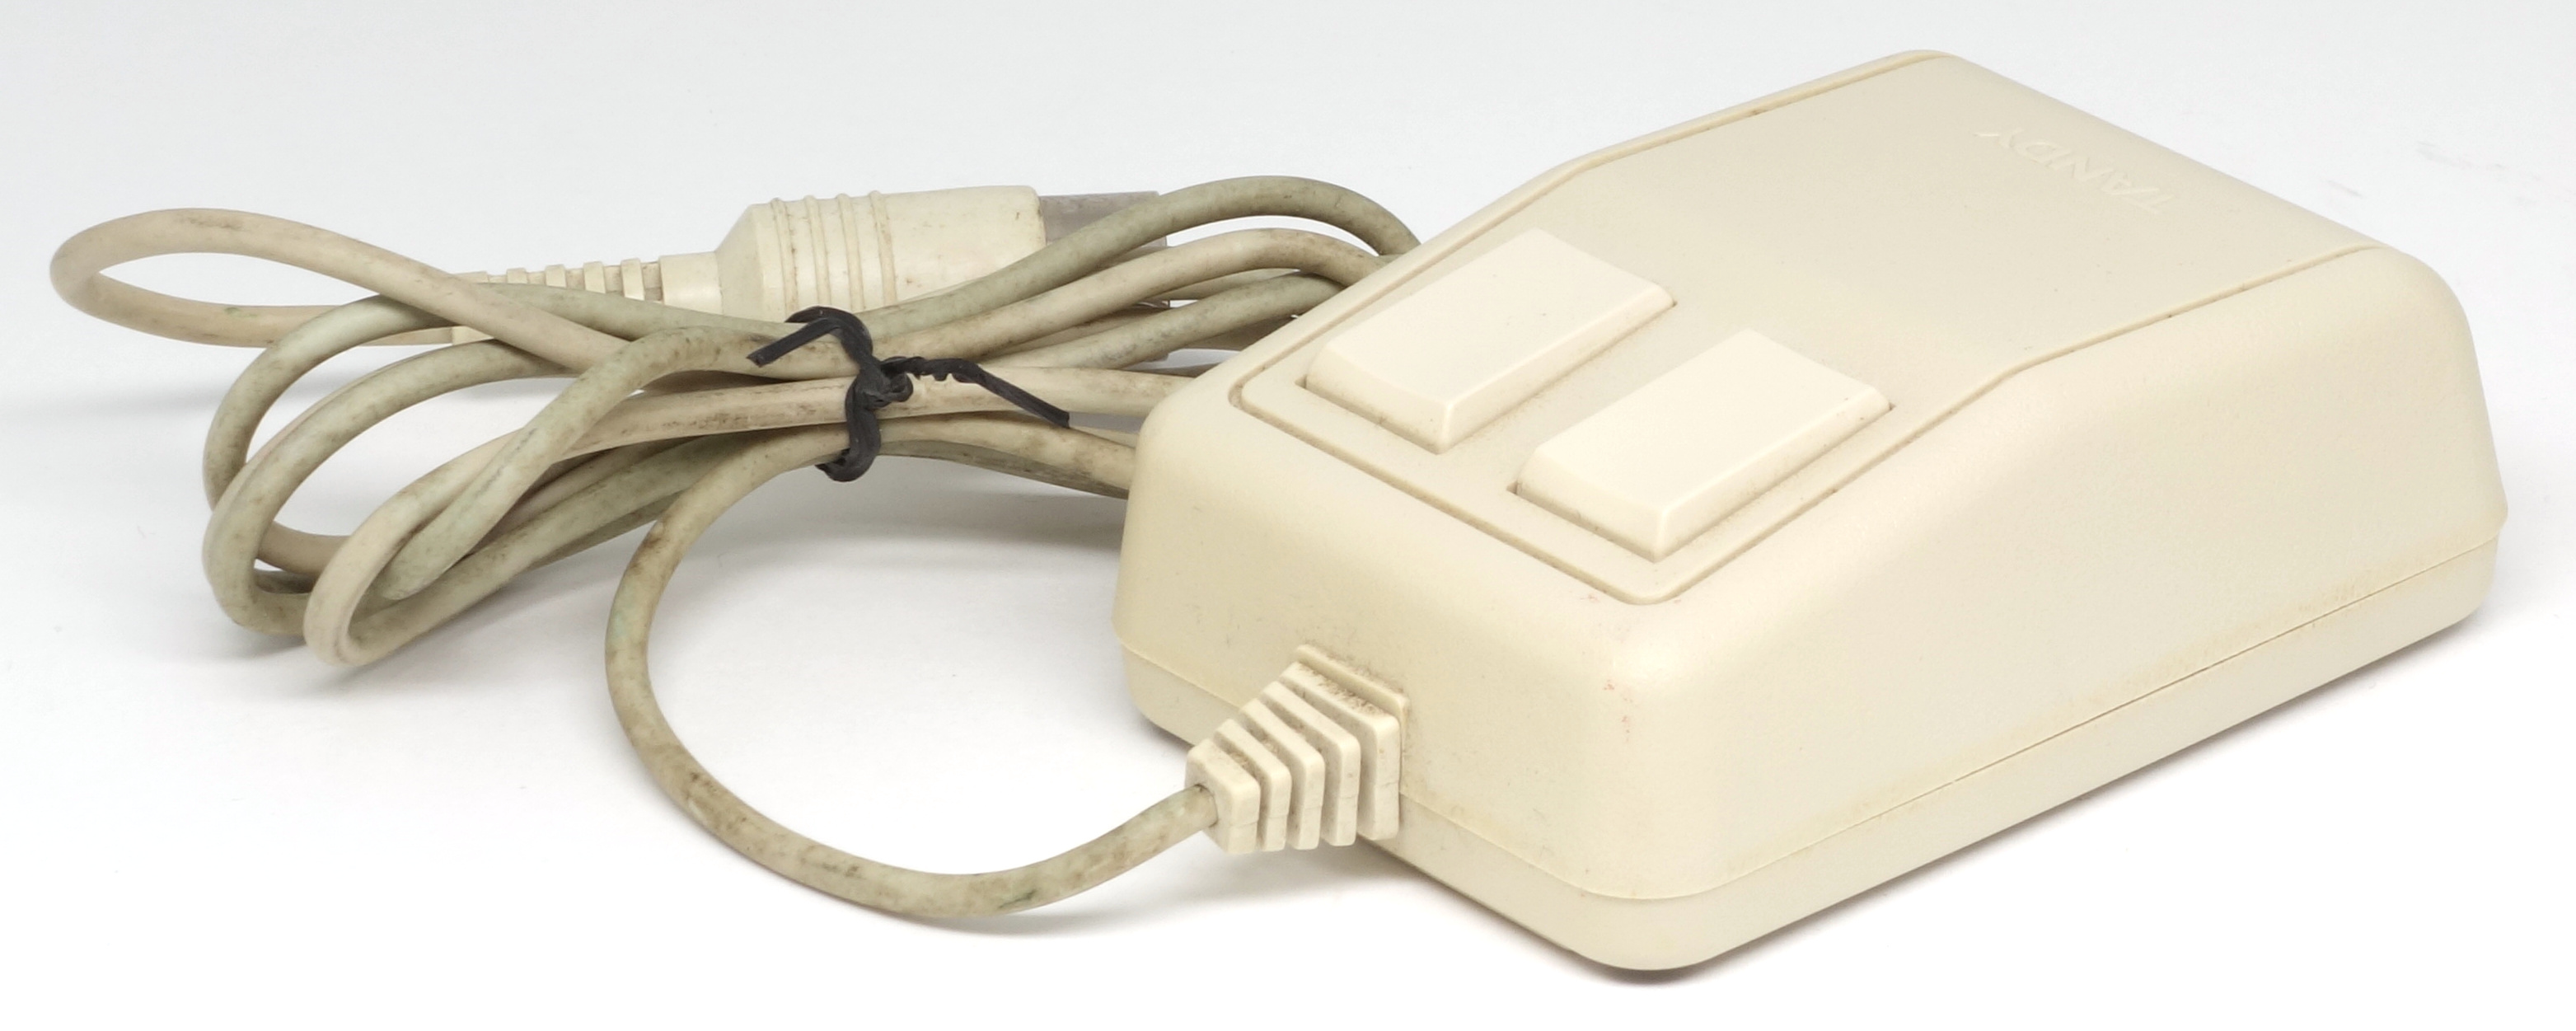
\includegraphics[scale=0.7]{1988_tandy_trs80_deluxe_mouse/pic_30.jpg}
    \caption{Tandy Deluxe Mouse}
    \label{fig:TandyDeluxeMousePic}
\end{figure}

\begin{figure}[h]
    \centering
    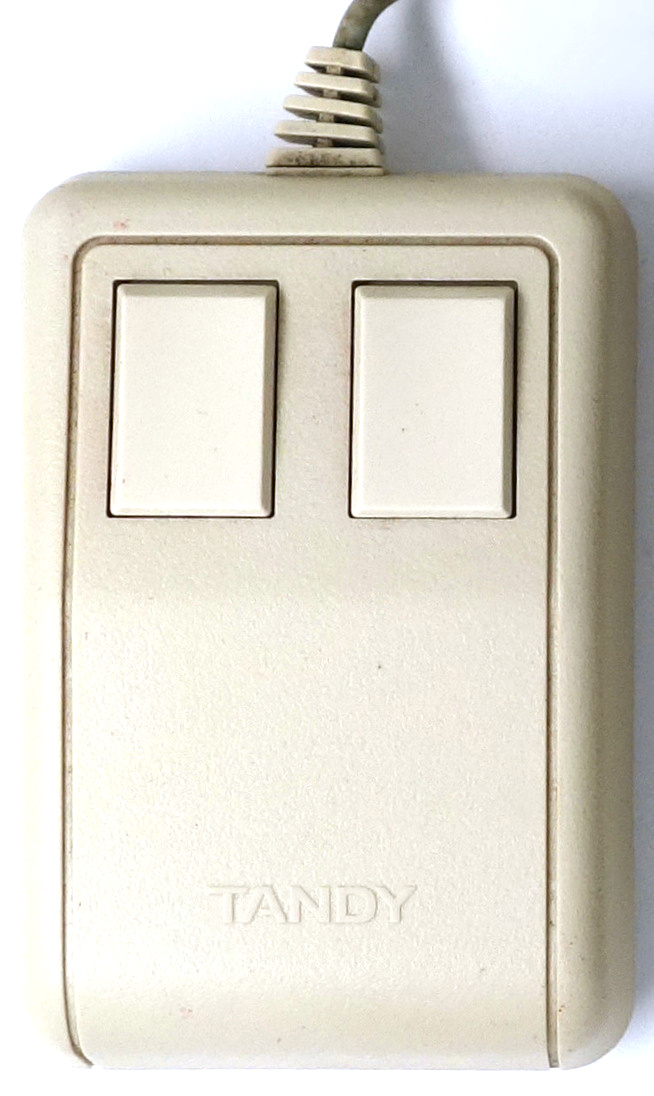
\includegraphics[scale=0.65]{1988_tandy_trs80_deluxe_mouse/top_60.jpg}
    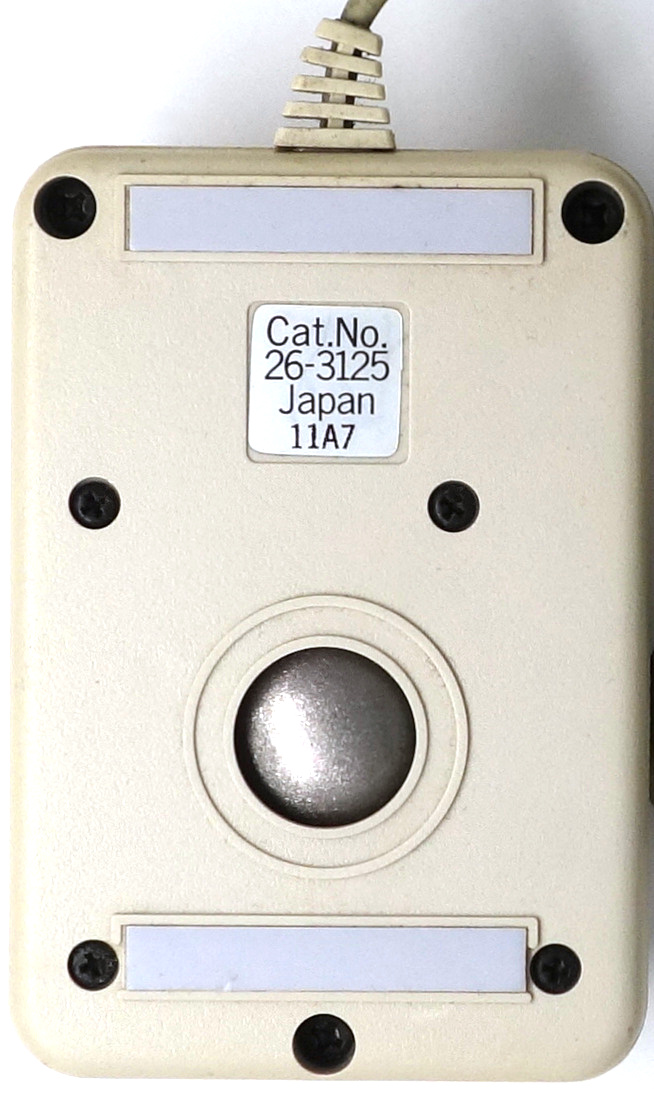
\includegraphics[scale=0.65]{1988_tandy_trs80_deluxe_mouse/bottom_30.jpg}
    \caption{Tandy Deluxe Mouse, top and bottom views}
    \label{fig:TandyDeluxeMouseTopAndBottom}
\end{figure}

Unlike its predecessor Color Mouse, the Tandy TRS-80 Deluxe Mouse has two buttons (fig. \ref{fig:TandyDeluxeMouseTopAndBottom}) and its begie body is rather typical for the mice of eighties \cite{hierophant}.

The bottom side shows exactly the same steel ball as the Color Mouse has, and the same lack of the latch ring which would allow removing the ball for cleaning. The only improvement is the appearance of low-friction rectangles that make it easier to move the mouse.

The mouse has a small size typical of the 80s (fig. \ref{fig:TandyDeluxeMouseSize}) and rather tall body.

\begin{figure}[h]
    \centering
    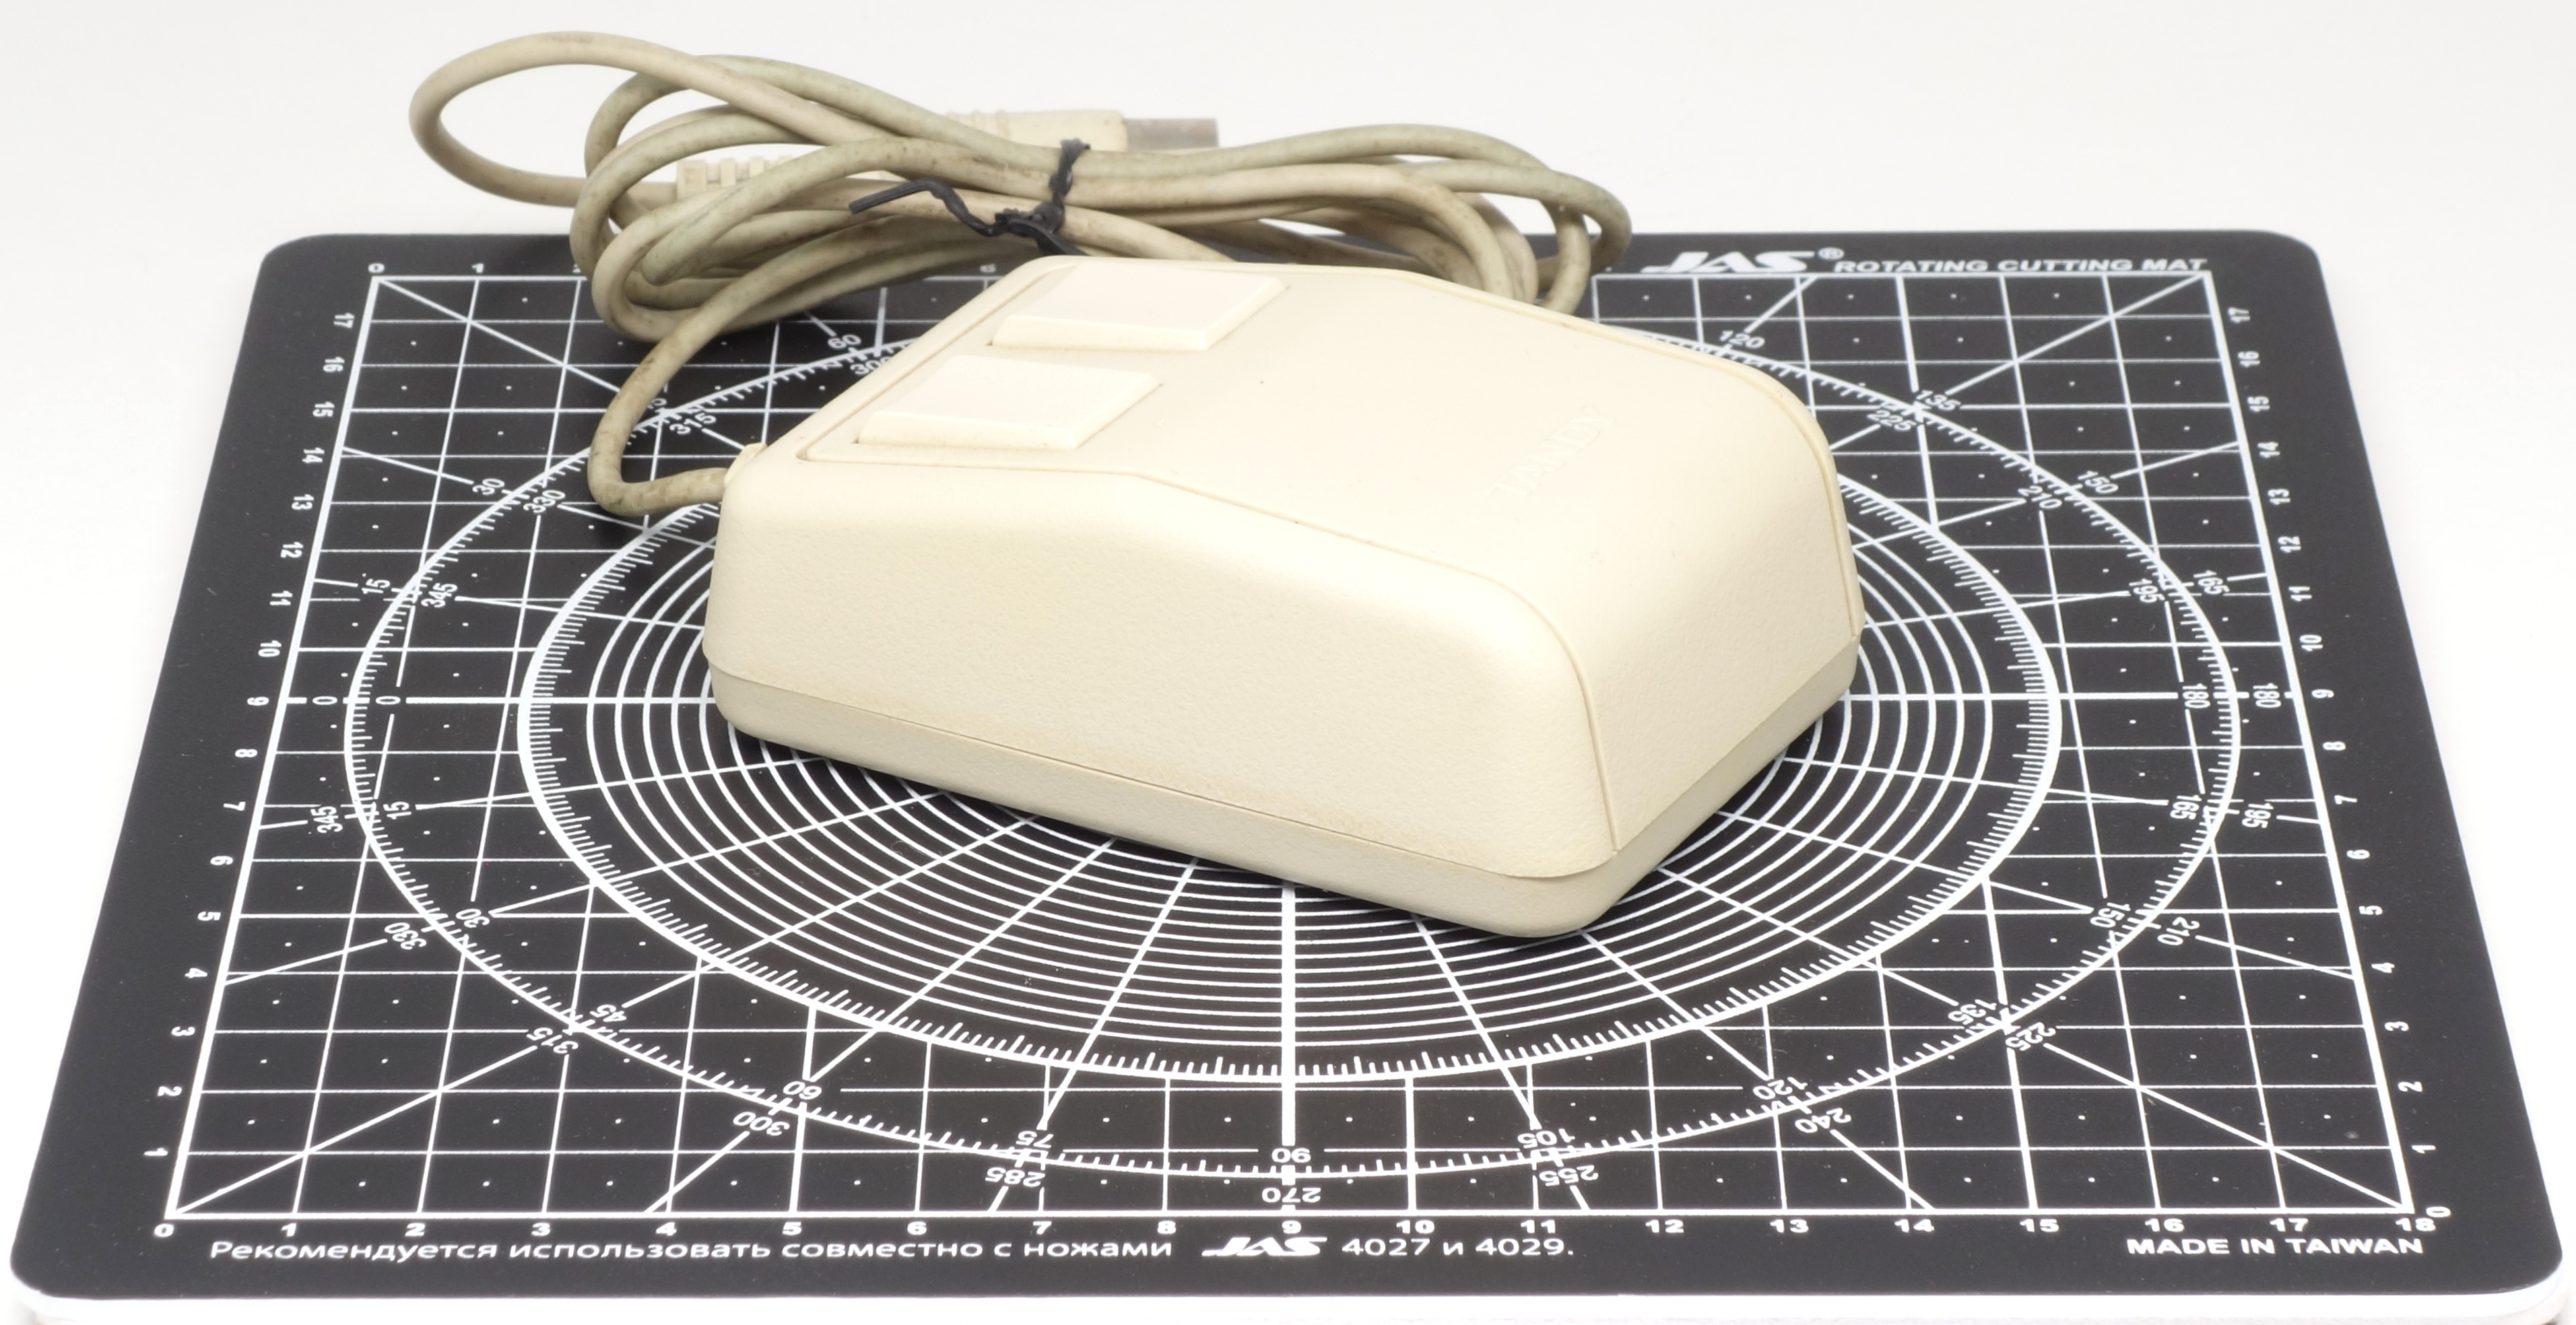
\includegraphics[scale=0.49]{1988_tandy_trs80_deluxe_mouse/size_15.jpg}
    \caption{Tandy Deluxe Mouse on a graduated pad with a grid step of 1~cm}
    \label{fig:TandyDeluxeMouseSize}
\end{figure}

The buttons on the Deluxe Mouse are large enough and slightly concave, which makes them comfortable enough to press with your fingers (fig. \ref{fig:TandyDeluxeMouseHand}). In general, the rounded edges of the body have a positive effect on ergonomics, but the shape of the body, typical among mice of the 80s, does not provide any significant support for the palm.

\begin{figure}[h]
    \centering
    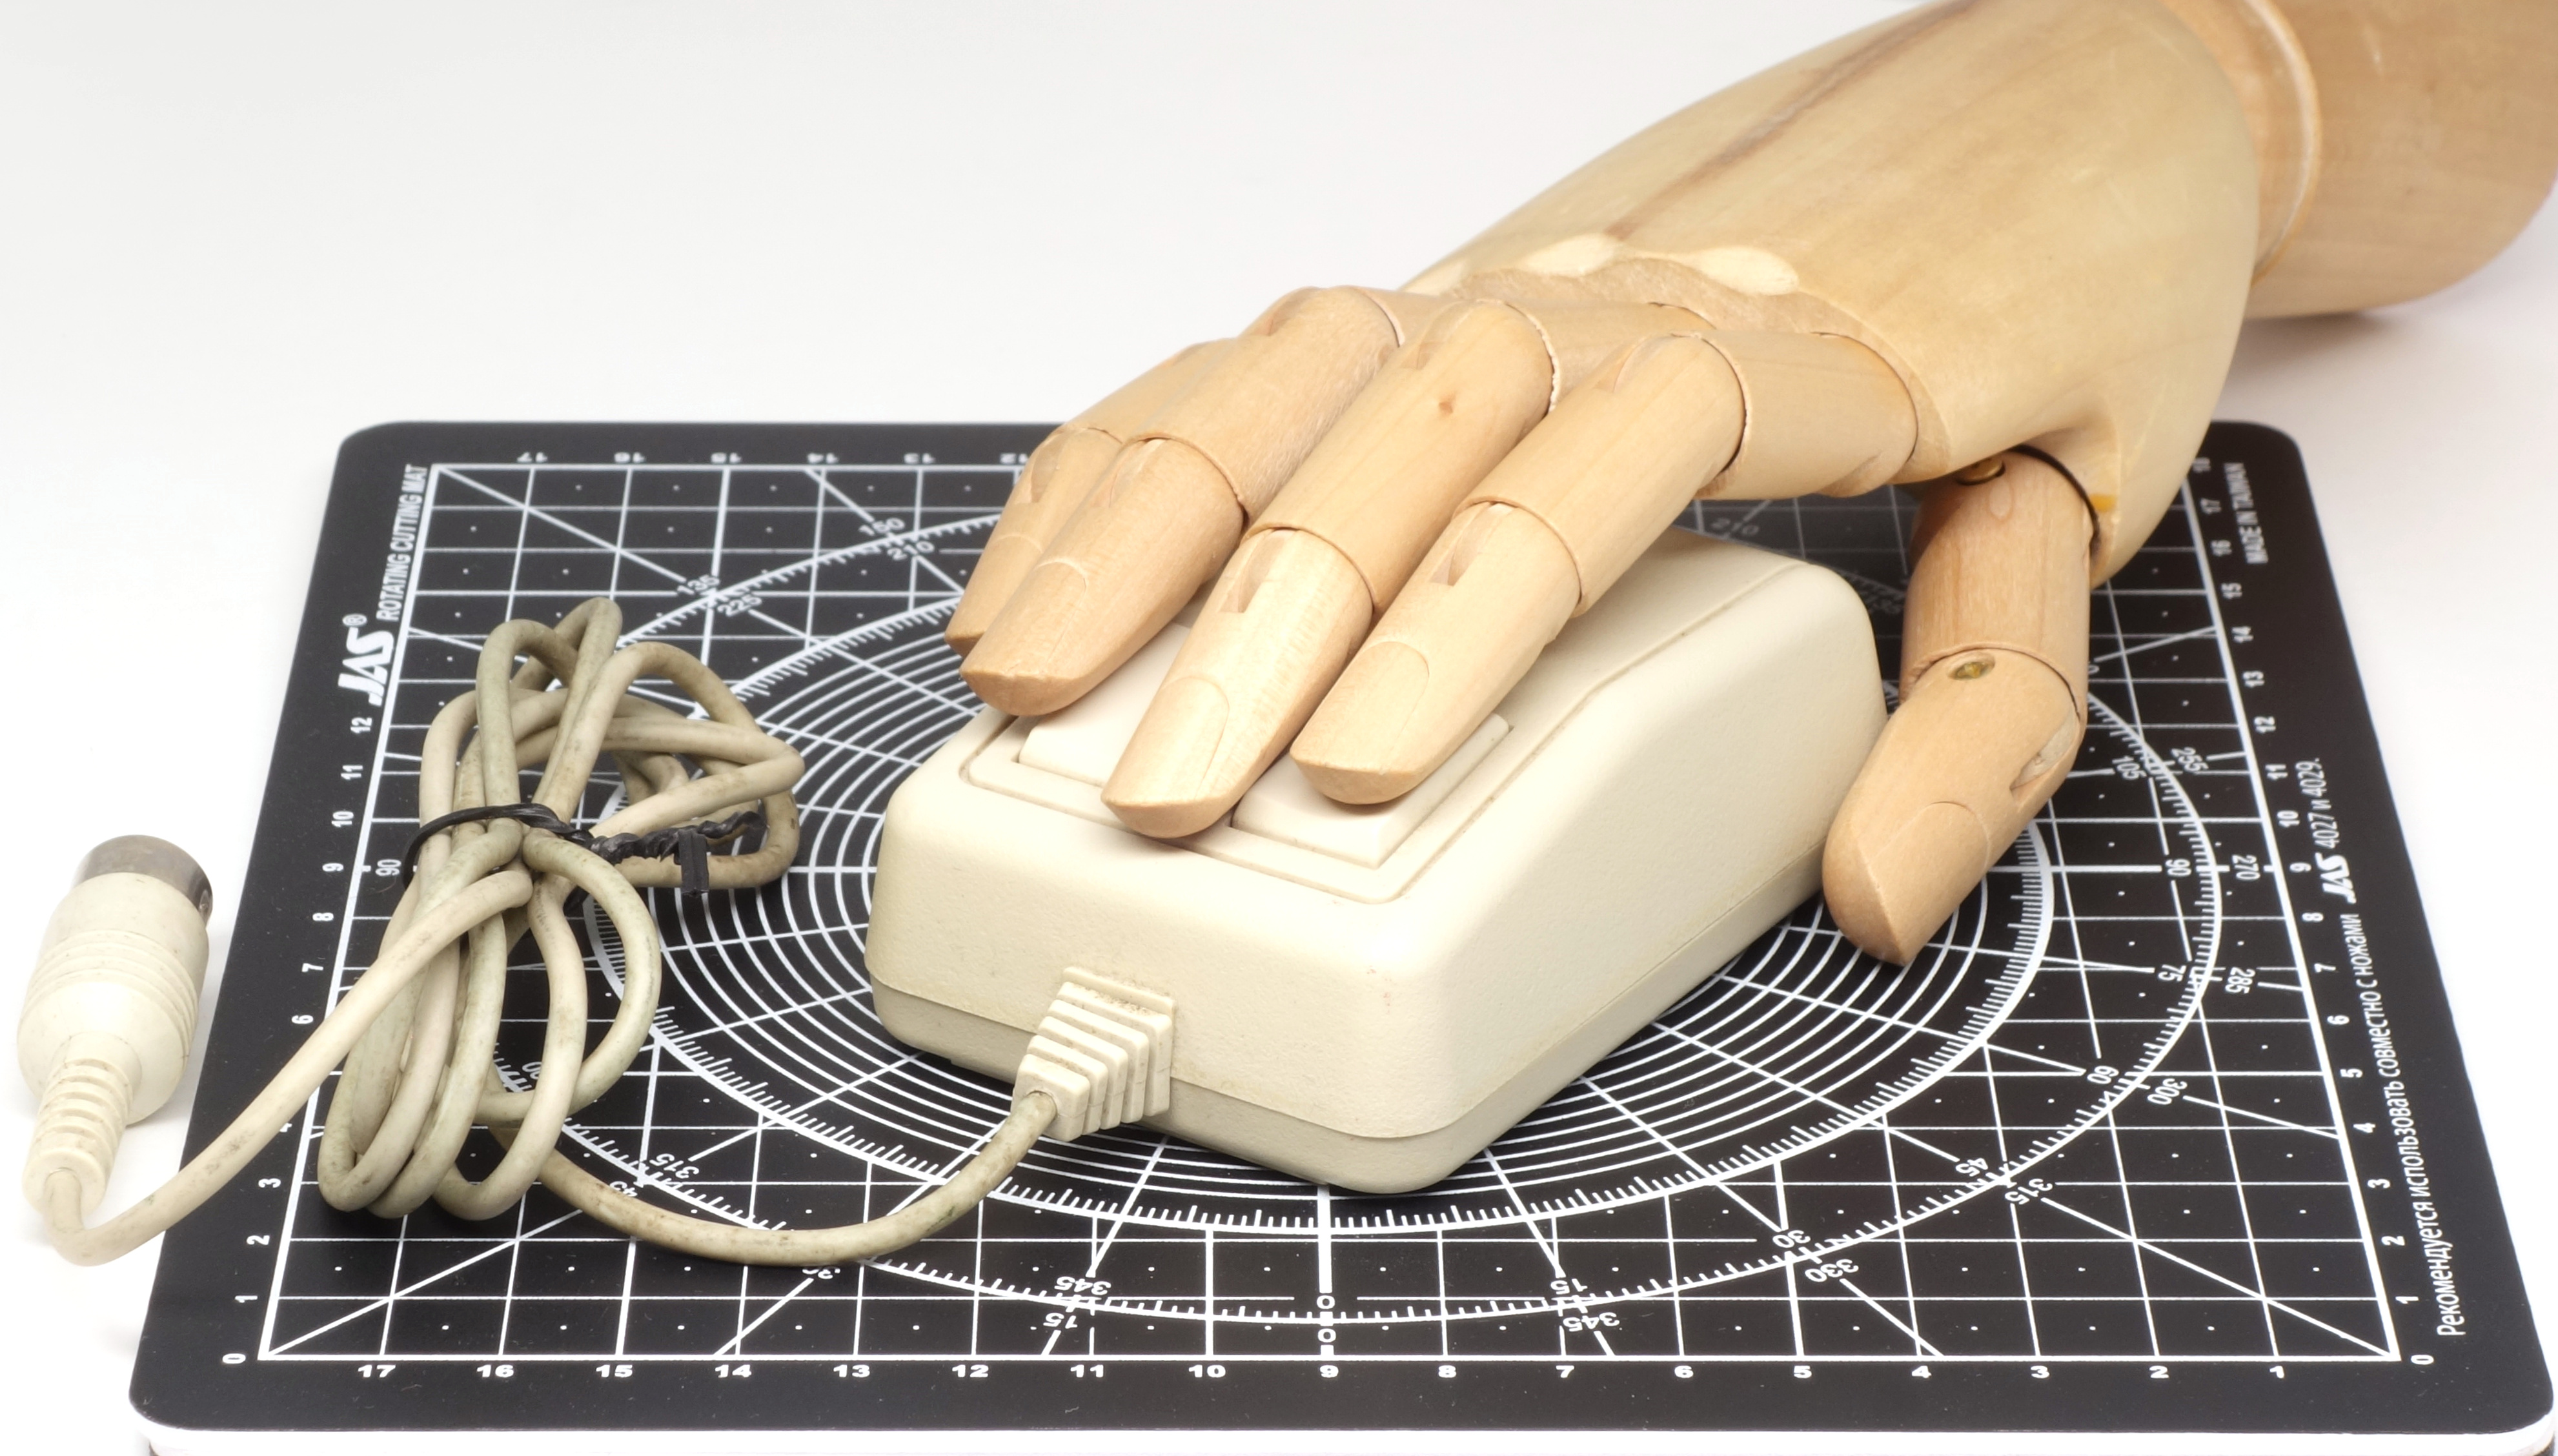
\includegraphics[scale=0.55]{1988_tandy_trs80_deluxe_mouse/hand_15.jpg}
    \caption{Tandy Deluxe Mouse with a human hand model}
    \label{fig:TandyDeluxeMouseHand}
\end{figure}

As mentioned, the mouse connects to the analog joystick port. As in the case of a joystick, information about each of the two coordinates is encoded in analog form, by the value of the electrical voltage on the corresponding connector pin. Same as Color Mouse, this mouse has resolution of 64 ``steps'' along each of two coordinate axes \cite{manual}, obviously caused by the limitations of the Tandy Color Computer analog-to-digital converter; drivers that allow using real analog joysticks to control mouse cursor were also showing poor positioning accuracy \cite{hierophant}.

\begin{figure}[h]
    \centering
    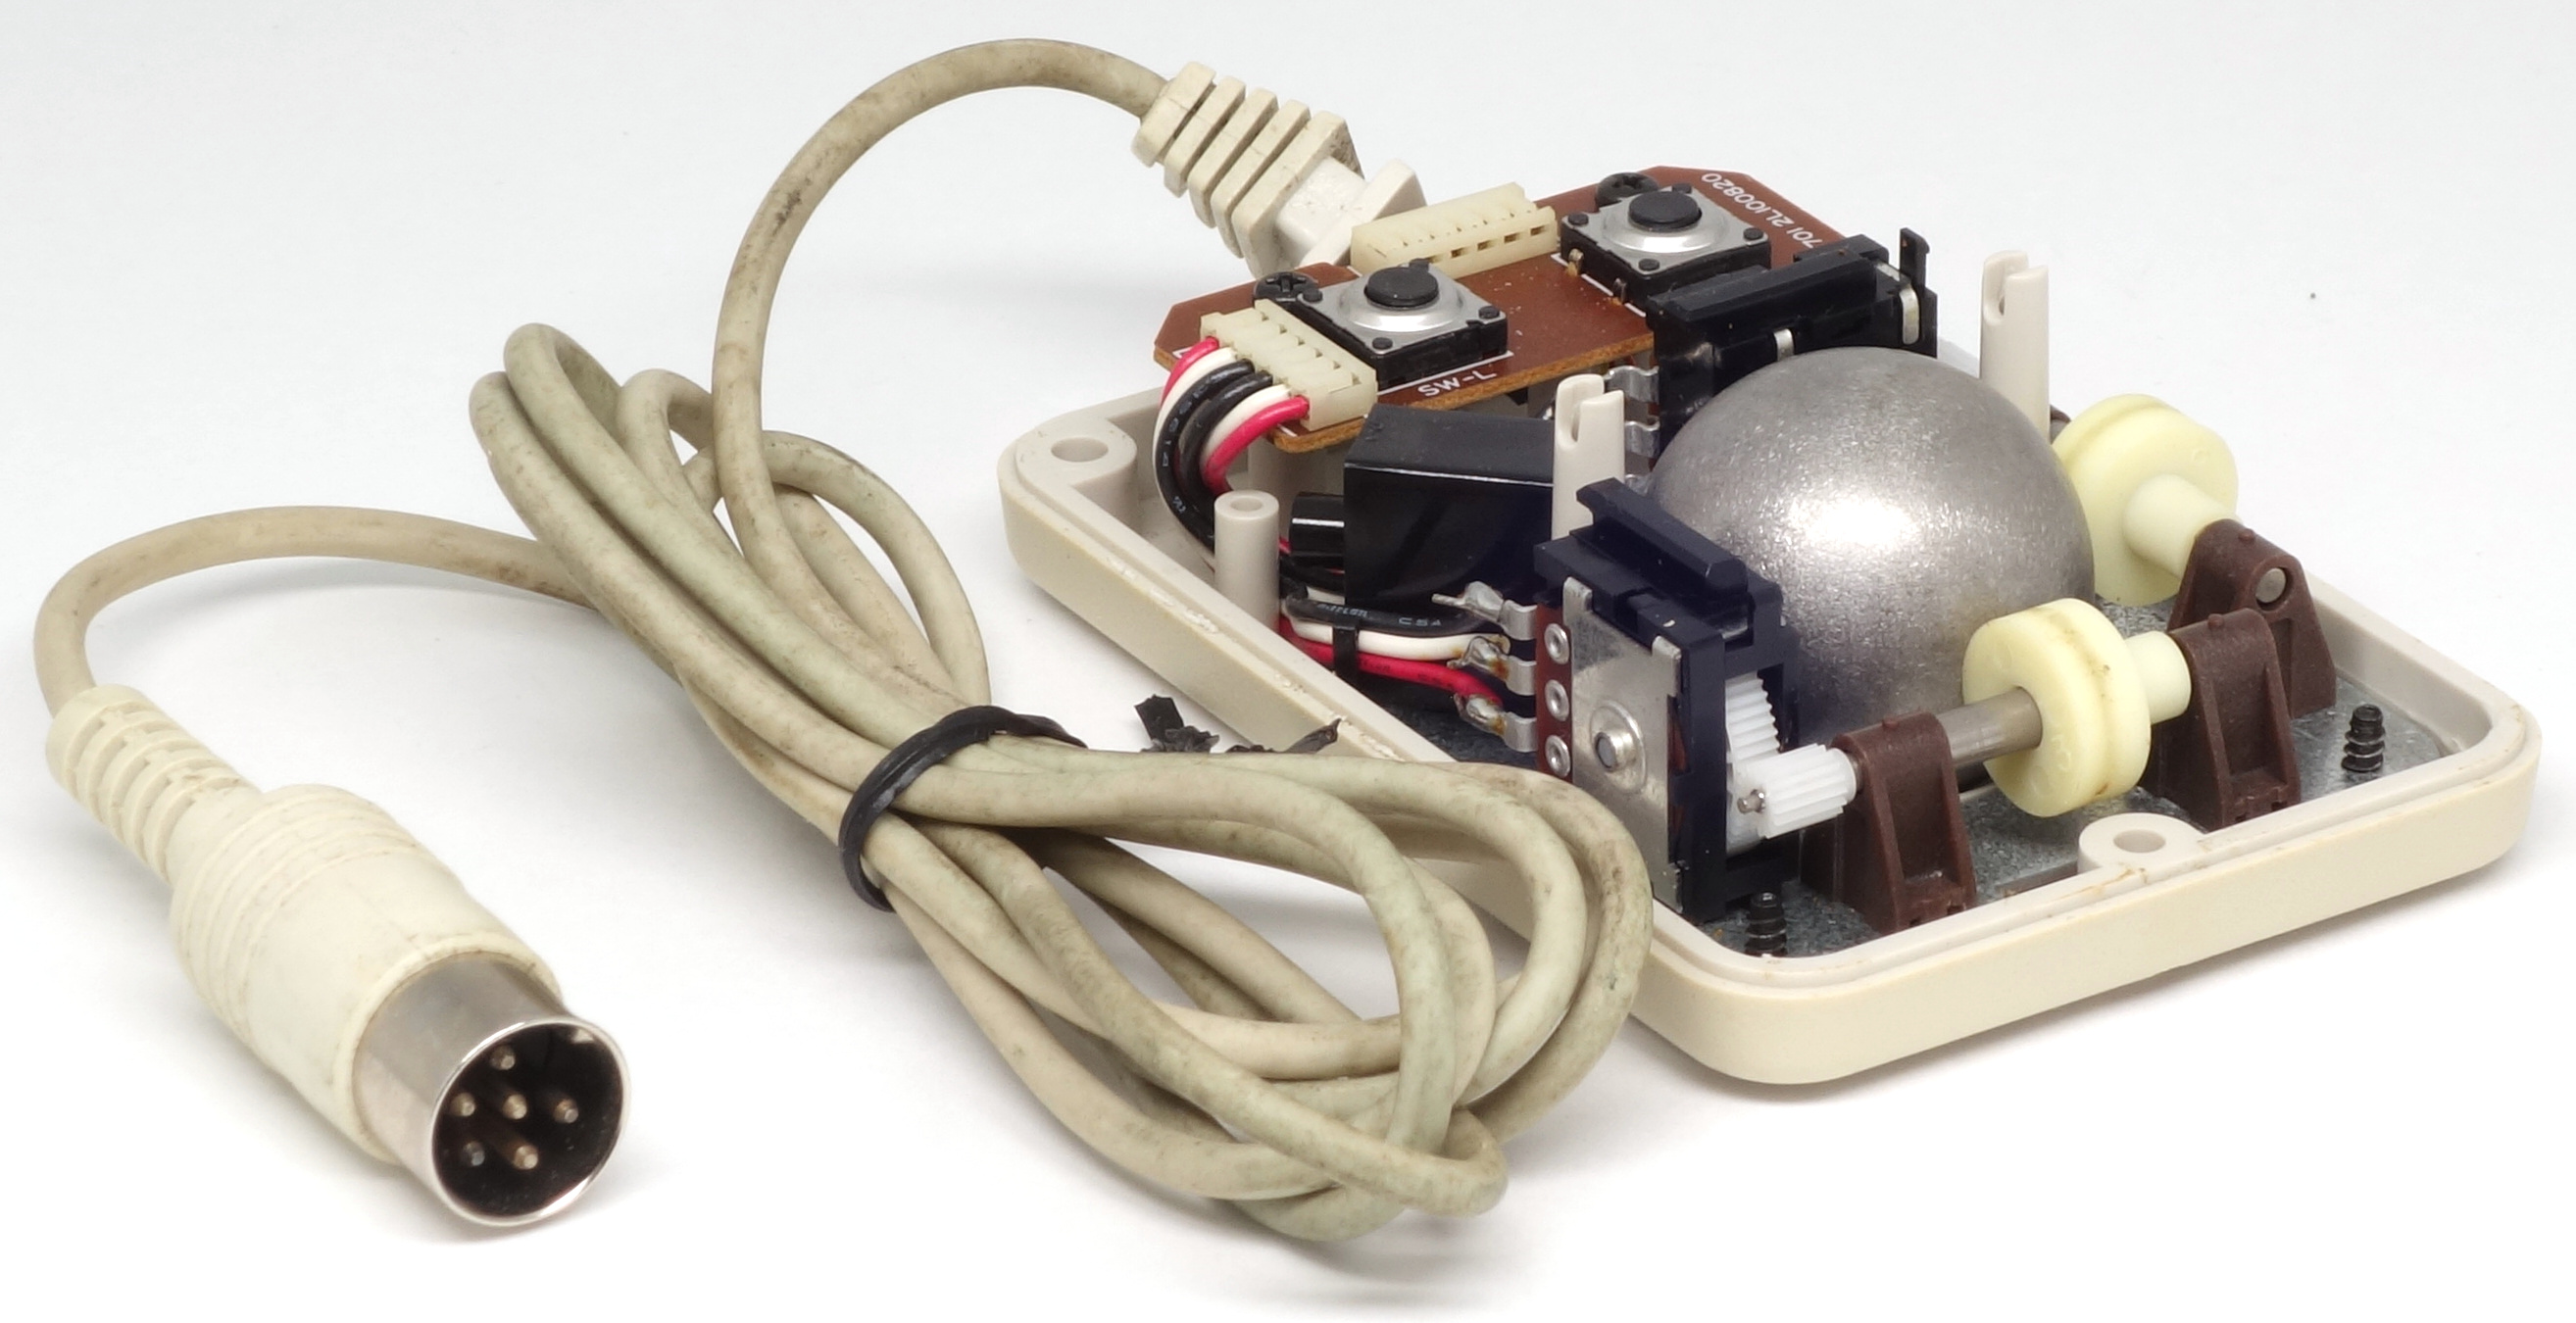
\includegraphics[scale=0.8]{1988_tandy_trs80_deluxe_mouse/inside_30.jpg}
    \caption{Tandy Deluxe Mouse disassembled}
    \label{fig:TandyDeluxeMouseInside}
\end{figure}

Disassembled mouse is shown in fig. \ref{fig:TandyDeluxeMouseInside}. Following the Color Mouse, Tandy Deluxe Mouse does not use contact or optomechanical encoders: instead, the ball transmits motion to a pair of potentiometers, just like an analog joystick stick does. Of course, this solution has significant drawbacks: the mouse does not allow calibration, and unlike the joystick, the mouse can't show user that its potentiometers have been moved to the middle position, which should correspond to the location in the center of the mousepad, or that they have reached the edje position. However, since Tandy Deluxe Mouse is an absolute coordinate pointing device, user can see location of the cursor on the screen and place the mouse on more or less appropriate part of the mousepad.

\begin{thebibliography}{9}
\bibitem {wiki} TRS-80 Color Computer -- Wikipedia \url{https://en.wikipedia.org/wiki/TRS-80_Color_Computer}
\bibitem {adv} 1988 Radio Shack Catalog. p. 177 \url{https://www.radioshackcatalogs.com/flipbook/1988_radioshack_catalog.html}, \url{https://web.archive.org/web/20210331035502/https://www.radioshackcatalogs.com/flipbook/catalogs/main/1988/177.jpg}
\bibitem {hierophant} Tandy Color Computer Mice - A Viable Alternative for Tandy 1000s without a Serial Port? January 21, 2016. -- \url{http://nerdlypleasures.blogspot.com/2016/01/tandy-color-computer-mice-viable.html}
\bibitem {manual} TANDY  COLOR COMPUTER TANDY 1000 SX / 1000 EX COLOR MOUSE Operational Manual \url{https://colorcomputerarchive.com/repo/Documents/Manuals/Hardware/Deluxe%20Color%20Mouse%20%28Tandy%29.pdf}
\end{thebibliography}
\end{document}
